\documentclass[11pt]{article}
\usepackage[margin=1in]{geometry}
\usepackage{amsmath,amssymb,booktabs,graphicx,hyperref,longtable,array}
\usepackage{caption}
\usepackage{float}
\title{A Voxel-Spacing-Aware Extension of PyRadiomics for Anisotropic Texture Analysis}
\author{Technical implementation audit generated from local source comparison}
\date{\today}
\begin{document}
\maketitle

\begin{abstract}
Radiomic texture features are frequently extracted from anisotropic CT and MRI acquisitions. Standard PyRadiomics texture computation enumerates voxel relationships in discrete index space, where a one-voxel offset along the slice direction is treated analogously to a one-voxel offset in-plane. When voxel spacing is anisotropic, these offsets can correspond to substantially different physical distances. A common workaround is isotropic resampling, but resampling couples geometric correction to interpolation-induced signal modification. This manuscript describes and audits a modified PyRadiomics implementation designed to preserve the gray levels supplied to texture computation while incorporating physical voxel spacing into selected texture operations. The central methodological idea is to separate geometric correction from interpolation-induced signal modification. GLCM receives voxel-spacing-aware feature-level angular aggregation; NGTDM receives a distance-weighted neighborhood mean; GLRLM, GLDM and GLSZM are computed after a finite-volume zero-order-hold representation of anisotropic voxel support. The implementation is opt-in, preserves standard PyRadiomics behavior when disabled, and is accompanied by synthetic validation of rounding error, computational expansion and comparison against isotropic resampling baselines.
\end{abstract}

\section{Introduction}
Medical images often have anisotropic voxel spacing, especially in clinical CT and MRI where through-plane spacing can differ markedly from in-plane spacing. Radiomic features extracted from such images may therefore conflate image texture, acquisition geometry, and preprocessing choices. PyRadiomics is a widely used radiomics library, but many texture matrices are computed using discrete offsets defined in index space. This is computationally natural, yet geometrically incomplete when a displacement of one voxel does not represent the same physical length along all axes.

\section{Motivation: anisotropy, interpolation and index-space texture bias}
Let voxel spacing be \(s=(\Delta_z,\Delta_y,\Delta_x)\). A discrete offset vector \(a=(a_z,a_y,a_x)\) corresponds to the physical offset length
\begin{equation}
d_a = \sqrt{(a_z\Delta_z)^2 + (a_y\Delta_y)^2 + (a_x\Delta_x)^2}.
\end{equation}
In an anisotropic volume, offsets such as \((1,0,0)\) and \((0,1,0)\) are both one index step but may be physically very different. Isotropic resampling addresses this geometric inconsistency by creating an isotropic grid, but it also interpolates intensities and modifies local spatial-frequency content. The modified implementation studied here follows a different design: preserve the gray levels supplied to texture computation and incorporate spacing into the interpretation, aggregation or finite-volume representation of voxel relationships.

\section{Overview of standard PyRadiomics texture computation}
Standard PyRadiomics builds texture matrices by enumerating neighbors or runs using discrete offsets derived from distance and dimensionality settings. Directional matrices may then be averaged or weighted according to existing weighting norms. Shape features already use physical spacing. First-order features primarily summarize intensity distributions and are less directly tied to neighborhood geometry, except for volume-scaled quantities such as Total Energy.

\section{Design principles of voxel-spacing-aware extraction}
The proposed design follows four principles. First, the gray levels supplied to texture computation are preserved. Second, no isotropic interpolation is introduced. Third, physical voxel spacing is used only where the mathematical structure of the descriptor admits a meaningful correction or finite-volume representation. Fourth, the new behavior is opt-in and must not alter standard PyRadiomics behavior when disabled.

For a set of non-zero offsets \(A\), let the index-space offset length be
\begin{equation}
\ell_a = \sqrt{a_z^2+a_y^2+a_x^2},
\end{equation}
and let the anisotropy-relative physical stretch be
\begin{equation}
r_a = \frac{d_a}{\ell_a}.
\end{equation}
Valid texture offsets exclude the zero vector and voxel spacings are strictly positive; therefore \(r_a>0\). The conceptual inverse-distance directional weights are
\begin{equation}
w_a = \frac{1}{r_a}, \qquad
W_a = \frac{w_a}{\sum_{b\in A} w_b}.
\end{equation}
In the implementation, GLCM uses \(1/\max(r_a,10^{-5})\) as a numerical floor. NGTDM computes \(r_a=d_a/(\ell_a+10^{-12})\) in the C backend and uses \(1/(r_a+10^{-6})\) for the local weighted mean. These constants are numerical safeguards only; they are negligible relative to valid non-zero offset stretches in the present extraction settings. These weights are not a claim of continuous-space radiomics. They are a discrete-grid correction for physically unequal offsets. For matrix families handled by finite-volume representation, anisotropic voxels are instead expanded by zero-order hold onto an isotropic subcell lattice; this replicates native gray levels and does not interpolate them.

\section{Software architecture and implementation}
The modified package adds frontend Python logic, a shared spacing utility, and C wrapper/backend functions. In the Python layer, feature classes inspect settings such as \texttt{weightingNorm='voxelSpacing'} or receive \texttt{voxelSpacing}. In the wrapper layer, \texttt{calculate\_ngtdm\_spacing} passes spacing arrays into C for NGTDM. Finite-volume GLRLM, GLDM and GLSZM are prepared in Python by repeat-factor calculation and zero-order-hold expansion before standard matrix construction. In the backend, physical distances are computed from discrete offsets and spacing where required. In the clean reproducibility package, the retained implementation snapshot contains the voxel-spacing-aware texture changes and excludes unrelated experimental preprocessing branches. Table~\ref{tab:modified-files} lists the core implementation files relevant to the method. Figure~\ref{fig:architecture} summarizes this flow.

All validation experiments reported here use segment-based, fully three-dimensional texture extraction with \texttt{force2D=False}; they are not two-dimensional or 2.5-dimensional texture calculations. Internally, SimpleITK images are converted to NumPy arrays in \((z,y,x)\) order, whereas SimpleITK reports spacing in \((x,y,z)\) order. The voxel-spacing-aware paths therefore use \texttt{GetSpacing()[::-1]} before applying spacing to array-index offsets or finite-volume repeat factors. Image direction/orientation matrices are not incorporated into the voxel-spacing-aware calculations; only voxel spacing magnitudes are used.

\begin{table*}[t]
\centering
\small
\begin{tabular}{p{0.19\textwidth}p{0.19\textwidth}p{0.19\textwidth}p{0.19\textwidth}p{0.19\textwidth}}
\toprule
file & affected family or layer & new parameters or terms & mathematical meaning & pr maturity \\
\midrule
base.py & Frontend/configuration & none detected & Configuration or utility support for optional spacing-aware behavior. & supporting \\
featureextractor.py & Frontend/configuration & weightingNorm & Configuration or utility support for optional spacing-aware behavior. & supporting \\
firstorder.py & First-order & voxelSpacing, weightingNorm & Volume-aware branch for Total Energy; most first-order features are not neighborhood geometry descriptors. & ancillary \\
glcm.py & GLCM & calculate\_glcm, compute\_offset\_distance, spacing\_utils, voxelSpacing, weightingNorm & Voxel-spacing-aware feature-level angular aggregation; co-occurrence enumeration remains native index-space. & conservative mature \\
gldm.py & GLDM & calculate\_gldm, spacing\_utils, voxelSpacing, weightingNorm & Finite-volume zero-order-hold GLDM construction; dependence size remains an integer matrix axis. & finite-volume mature \\
glrlm.py & GLRLM & calculate\_glrlm, spacing\_utils, voxelSpacing, weightingNorm & Finite-volume zero-order-hold GLRLM construction; run length remains an integer matrix axis. & finite-volume mature \\
glszm.py & GLSZM & calculate\_glszm, spacing\_utils, voxelSpacing, weightingNorm & Finite-volume zero-order-hold GLSZM construction; zone size remains an integer matrix axis. & finite-volume mature \\
ngtdm.py & NGTDM & calculate\_ngtdm, calculate\_ngtdm\_spacing, voxelSpacing, weightingNorm & Distance-weighted neighborhood averaging before NGTDM gray-level accumulation. & strong descriptor extension \\
schemas/schemaFuncs.py & Frontend/configuration & voxelSpacing & Configuration or utility support for optional spacing-aware behavior. & supporting \\
spacing\_utils.py & Shared spacing utility & compute\_offset\_distance, spacing\_utils & Configuration or utility support for optional spacing-aware behavior. & supporting \\
src/\_cmatrices.c & C matrix backend/wrapper & calculate\_glcm, calculate\_gldm, calculate\_glrlm, calculate\_glszm, calculate\_ngtdm, calculate\_ngtdm\_spacing & C wrapper/backend support for standard matrix construction and spacing-aware NGTDM. & backend support \\
src/cmatrices.c & C matrix backend/wrapper & calculate\_glcm, calculate\_gldm, calculate\_glrlm, calculate\_glszm, calculate\_ngtdm, calculate\_ngtdm\_spacing & C backend support for standard matrices and spacing-aware NGTDM local weighting. & backend support \\
src/cmatrices.h & C matrix backend/wrapper & calculate\_glcm, calculate\_gldm, calculate\_glrlm, calculate\_glszm, calculate\_ngtdm, calculate\_ngtdm\_spacing & Exported matrix signatures, including spacing-aware NGTDM. & backend support \\
\bottomrule
\end{tabular}
\caption{Core changed implementation files relevant to voxel-spacing-aware radiomics. This table is methodological, not an exhaustive \texttt{git diff --stat} listing.}
\label{tab:modified-files}
\end{table*}

\section{Feature-family-specific modifications}
\subsection{GLCM}
The GLCM modification is conservative. Co-occurrence pairs are still enumerated in native index space, producing directional matrices \(P_a(i,j)\). The implementation does not first combine these matrices into a single weighted matrix. Instead, each GLCM feature \(f\) is computed per direction and the final angular aggregation is weighted:
\begin{equation}
F_f = \sum_{a\in A} W_a f(P_a).
\end{equation}
This distinction matters because, for non-linear GLCM features, \(\sum_a W_a f(P_a)\neq f(\sum_a W_aP_a)\). The modification should therefore be described as voxel-spacing-aware feature-level angular aggregation, not as weighted matrix fusion and not as a full physical-space GLCM.

\subsection{GLRLM}
GLRLM is computed after finite-volume zero-order-hold expansion when \texttt{weightingNorm='voxelSpacing'} is enabled in anisotropic images. Let \(h=\min(\Delta_z,\Delta_y,\Delta_x)\) and
\begin{equation}
q_k=\mathrm{round}\left(\frac{\Delta_k}{h}\right), \qquad k\in\{z,y,x\}.
\end{equation}
The native binned image is expanded by repeating each voxel \(q_k\) times along axis \(k\), creating \(\tilde I=\mathrm{ZOH}(I;q_z,q_y,q_x)\). The represented spacing and relative spacing error are therefore
\begin{equation}
\Delta_k^{*}=q_kh,\qquad
e_k=\frac{\Delta_k^{*}-\Delta_k}{\Delta_k}.
\end{equation}
Standard GLRLM construction is then applied to \(\tilde I\). Run length remains an integer count, but it counts isotropic physical subcells rather than anisotropic native voxels. This integer representation is the main mathematical approximation of the finite-volume method: for example, \(2.5{:}1{:}1\) is represented as \(2{:}1{:}1\), giving \(e_z=-20.0\%\), whereas \(3.5{:}1{:}1\) is represented as \(4{:}1{:}1\), giving \(e_z=+14.3\%\). The implementation guards the product \(q_zq_yq_x\) through \texttt{maximumExpansionFactor}; the finite-volume paths log \(q_k\), \(\Delta_k^{*}\), \(e_k\), and expanded shape, and emit a warning containing \(R\) when the expansion factor exceeds 8.

\subsection{NGTDM}
NGTDM is a stronger descriptor-level extension because the descriptor depends explicitly on a local neighborhood mean. The modified backend preserves native discrete neighborhood topology but replaces the unweighted local mean by
\begin{equation}
\bar I(x) = \frac{\sum_{a\in N(x)} I(x+a)w_a}{\sum_{a\in N(x)} w_a}.
\end{equation}
The usual gray-level accumulation then uses \(|I(x)-\bar I(x)|\). This is conceptually strong because neighborhood averaging naturally admits inverse-distance physical weighting.

\subsection{GLDM}
GLDM is also computed on the finite-volume zero-order-hold representation \(\tilde I\). Standard dependence counting is then applied without fractional dependence weights. Dependence size remains an integer count, avoiding the earlier weighted-dependence prototype in which a continuous value had to be rounded back to a matrix axis.

\subsection{GLSZM}
GLSZM is topology-based: it describes connected zones of equal gray level. Under anisotropic \texttt{voxelSpacing}, the standard connected-component algorithm is applied to the finite-volume zero-order-hold representation \(\tilde I\). Zone size remains an integer count, but it counts isotropic subcells rather than anisotropic native voxels. This is preferable to post-hoc volume scaling because matrix construction and feature formulas remain standard after representation.

\subsection{Shape and first-order considerations}
Shape features already use image spacing in standard PyRadiomics. First-order features are mostly intensity-distribution descriptors. The observed Total Energy branch is ancillary and should not be grouped with texture-neighborhood corrections.

\subsection{Finite-volume expansion safeguards}
For finite-volume families, the computational expansion factor is
\begin{equation}
R=q_zq_yq_x,
\end{equation}
and the expanded lattice size is
\begin{equation}
N_{\mathrm{expanded}}=(N_zq_z)(N_yq_y)(N_xq_x).
\end{equation}
The current implementation computes the expanded shape before allocating the expanded image and mask. The shared helper exposes a \texttt{maximumExpansionFactor} guard on \(R\), with default value 1000; the finite-volume feature classes call this helper with its default value. The implementation records represented-spacing metadata in logger messages and emits warnings when \(\max_k |e_k|>10\%\) or \(R>8\). It does not currently enforce an absolute \(N_{\mathrm{expanded}}\) memory guard at library level. For routine use, we recommend also reporting \(N_{\mathrm{expanded}}\) to the user before allocation and requiring explicit user confirmation or a hard stop for very large expansions such as \(R>16\) or user-defined memory limits.

\begin{table*}[t]
\centering
\small
\begin{tabular}{p{0.16\textwidth}p{0.16\textwidth}p{0.16\textwidth}p{0.16\textwidth}p{0.16\textwidth}p{0.16\textwidth}}
\toprule
feature family & standard mathematical dependency & anisotropy problem & modification type & base definition changes & pr maturity \\
\midrule
GLCM & Directional co-occurrence offsets & One index step can represent unequal physical distances & Voxel-spacing-aware feature-level angular aggregation & No & Conservative mature \\
GLRLM & Directional runs counted in voxels & Native voxel counts underrepresent thick-slice physical support & Finite-volume zero-order-hold matrix construction & Yes opt-in & Finite-volume mature \\
NGTDM & Local neighborhood mean & Unweighted mean treats near and far anisotropic neighbors equally & Distance-weighted neighborhood averaging & Yes & Strong descriptor extension \\
GLDM & Dependence size as integer neighbor count & Dependent-neighbor counts are tied to anisotropic native voxel support & Finite-volume zero-order-hold matrix construction & Yes opt-in & Finite-volume mature \\
GLSZM & Connected zones/topology & Zone size in native voxels differs from physical zone support & Finite-volume zero-order-hold matrix construction & Yes opt-in & Finite-volume mature \\
First-order & Intensity histogram and scalar intensity moments & Mostly not neighborhood-direction dependent; total energy is volume-scaled & Ancillary voxel-volume handling only & Mostly no & Ancillary \\
Shape & Mesh/voxel geometry descriptors & Standard PyRadiomics already uses spacing for shape geometry & No new texture-mode correction & No & Standard \\
\bottomrule
\end{tabular}
\caption{Feature-family classification for voxel-spacing-aware extraction.}
\label{tab:family-classification}
\end{table*}

\section{Mathematical formulation}
The common mathematical object is the physical offset length \(d_a\). For GLCM, \(d_a\) changes the feature-level angular aggregation. For NGTDM, \(d_a\) changes the neighborhood mean. For GLRLM, GLDM and GLSZM, anisotropic voxel support is represented by finite-volume zero-order-hold expansion before standard matrix construction.

\begin{table*}[t]
\centering
\small
\begin{tabular}{p{0.32\textwidth}p{0.32\textwidth}p{0.32\textwidth}}
\toprule
family & equation & interpretation \\
\midrule
GLCM & $F_f=\sum_a W_a f(P_a)$ & Directional co-occurrences are enumerated on the native grid; each feature is computed per direction before weighted angular aggregation. \\
GLRLM & $R=\mathrm{GLRLM}(\tilde I)$ & Runs remain integer counts on the finite-volume lattice. \\
NGTDM & $\bar I(x)=\frac{\sum_{a\in N(x)} I(x+a)w_a}{\sum_{a\in N(x)}w_a}$ & Neighborhood mean is a true descriptor-level distance-weighted average. \\
GLDM & $G=\mathrm{GLDM}(\tilde I)$ & Dependence size remains an integer count on the finite-volume lattice. \\
GLSZM & $Z=\mathrm{GLSZM}(\tilde I)$ & Zone size remains an integer count on the finite-volume lattice. \\
\bottomrule
\end{tabular}
\caption{Mathematical summary of supported or considered spacing-aware operations.}
\label{tab:math-summary}
\end{table*}

\section{Compatibility with IBSI/PyRadiomics workflows}
Backward compatibility depends on default-off behavior. When the new mode is disabled, calls should route to the standard PyRadiomics implementation. The modified NGTDM and finite-volume matrix families should not be claimed as IBSI-compliant replacements; they are opt-in extensions. GLCM can be documented as optional anisotropy-aware feature-level angular aggregation.

\begin{table*}[t]
\centering
\small
\begin{tabular}{p{0.32\textwidth}p{0.32\textwidth}p{0.32\textwidth}}
\toprule
topic & implication & suggested wording \\
\midrule
Backward compatibility & Preserve original behavior unless the opt-in spacing-aware mode is enabled. & Use explicit parameter naming and default-off behavior. \\
IBSI implications & Modified NGTDM and finite-volume matrix families are not standard IBSI definitions. & Label as extensions rather than replacements. \\
Semantic risk & Finite-volume expansion changes the matrix construction domain. & Document zero-order-hold representation and expansion factors. \\
Documentation wording & Avoid claims of continuous-space radiomics. & Use native gray levels preserved, physical offset weighting and finite-volume representation. \\
\bottomrule
\end{tabular}
\caption{Compatibility and limitations.}
\label{tab:compatibility}
\end{table*}

\section{Additional software validation}
Three supplementary validation experiments quantify the main implementation risks: finite-volume rounding, computational expansion and non-equivalence to resampling. The validation tables and figures are distributed with the experiment outputs, including per-feature CSV tables for resampling comparisons.

\begin{table}[htbp]
\centering
\small
\caption{Additional software-validation summary.}
\begin{tabular}{p{0.17\linewidth}p{0.22\linewidth}p{0.18\linewidth}p{0.18\linewidth}p{0.17\linewidth}}
\toprule
Experiment & Main comparison & Key metric & Main result & Interpretation \\
\midrule
Resampling baseline comparison & Voxel-spacing-aware extraction vs native and isotropic resampling & Median relative difference; correlation & VS median relative difference vs native 0.307; linear resampling 0.304. & VS behaves as a distinct interpolation-free alternative. \\
Computational profiling & Spacing ratio and ROI size & Runtime vs expansion factor & Observed up to R=7; maximum completed runtime 1.74 s. & Cost scales with finite-volume expansion; warnings are advisable for high R. \\
Rounding sensitivity & Integer vs non-integer spacing ratios & Relative represented-spacing error & Maximum tested relative z-spacing error 0.2. & Non-integer ratios are approximated by integer repeat factors. \\
Binning sensitivity & binWidth 5, 10, 25, 50 & Median relative difference & VS vs native median relative difference range 0.145-0.233. & Discretization interacts with feature-level differences and should be reported. \\
\bottomrule
\end{tabular}
\end{table}


\subsection{Finite-volume rounding sensitivity}
The finite-volume representation was tested on spacing ratios \(1{:}1{:}1\), \(2{:}1{:}1\), \(2.5{:}1{:}1\), \(3{:}1{:}1\), \(3.5{:}1{:}1\), \(5{:}1{:}1\) and \(5.5{:}1{:}1\). The validation output records \(q_k\), \(\Delta_k^{*}\), \(e_k\) and \(R\). Integer ratios had zero represented-spacing error. The two most important non-integer examples were \(2.5{:}1{:}1\rightarrow2{:}1{:}1\), with \(e_z=-20.0\%\), and \(3.5{:}1{:}1\rightarrow4{:}1{:}1\), with \(e_z=+14.3\%\). Across adjacent spacing-ratio comparisons, the largest family-level median relative feature difference was 0.167 for GLSZM and the lowest Spearman correlation was 0.900 for NGTDM. These results do not remove the integer-rounding limitation, but they quantify it and make the approximation auditable. The adjacent integer comparisons also provide a low-cost floor/ceil sensitivity check around non-integer ratios, supporting round as the minimum absolute represented-spacing error choice under the current integer-repeat model.

\subsection{Computational profiling and stress testing}
Runtime and memory profiling used three synthetic volume sizes: \(16\times64\times64\), \(32\times96\times96\) and \(48\times128\times128\). The corresponding native ROI sizes were 12,126, 50,328 and 139,028 voxels. Tested expansion factors were \(R=1,2,3,5\) and an adverse axis case with \(R=7\). The most demanding completed case used a \(48\times128\times128\) input with spacing \(0.7{:}0.7{:}5.0\), producing \(q=(1,1,7)\), an expanded lattice of \(48\times128\times896\), 973,196 ROI voxels after expansion, a runtime of 1.74 s and a peak memory estimate of 90.55 MB. Median peak memory increased from 2.83 MB at \(R=1\) to 13.56 MB at \(R=7\), while maximum observed runtime remained below 1.75 s in the tested synthetic setting. These data support a moderate-cost claim only for the tested sizes and expansion factors; larger clinical volumes should use the pre-allocation \(N_{\mathrm{expanded}}\) estimate and configured limits.

\subsection{Comparison with isotropic resampling}
The resampling baseline compared native extraction, nearest-neighbor resampling, linear resampling, B-spline resampling and voxel-spacing-aware extraction on the same synthetic image family. The per-feature supplementary table contains one row per feature with native value, comparison value, absolute difference, relative difference and method columns for nearest, linear, B-spline and spacing-aware extraction. Relative to native extraction, nearest-neighbor resampling changed 192/225 features (85.3\%), linear and B-spline resampling changed 225/225 features (100\%), and voxel-spacing-aware extraction changed 192/225 features (85.3\%). The median of family-level median relative differences was 0.333 for nearest-neighbor resampling, 0.304 for linear resampling, 0.302 for B-spline resampling and 0.307 for voxel-spacing-aware extraction. Minimum method-level Spearman correlations were 0.900 for nearest-neighbor and voxel-spacing-aware extraction and 0.800 for linear and B-spline resampling. Thus, the spacing-aware method is not equivalent to resampling: it yields differences of comparable magnitude while preserving native gray levels rather than creating interpolated intensities. Figure~\ref{fig:resampling-family-differences} summarizes the family-level distributions.

\section{Limitations and known implementation risks}
The principal mathematical limitation is finite-volume integer rounding. When spacing ratios are non-integer, the represented spacing \(\Delta_k^{*}\) can differ from the acquired spacing \(\Delta_k\), and this error should be reported with the extracted features, logs or validation metadata. The second limitation is memory scaling: zero-order-hold expansion preserves native gray values but increases array size by \(R\). The third limitation is scope: the validation experiments are synthetic and designed to test software behavior, not to establish clinical superiority. The modified NGTDM and finite-volume matrix families should therefore be described as opt-in PyRadiomics extensions rather than IBSI-compliant replacements.

\section{Recommendations for upstream PyRadiomics integration}
An upstream pull request should be staged around opt-in behavior and backward compatibility. GLCM can be proposed as the most conservative feature-level angular-aggregation correction. NGTDM can be proposed as a well-motivated descriptor extension. GLRLM, GLDM and GLSZM can be proposed as finite-volume zero-order-hold matrix extensions, with explicit documentation that native gray levels are replicated rather than interpolated.

\begin{table*}[t]
\centering
\small
\begin{tabular}{p{0.32\textwidth}p{0.32\textwidth}p{0.32\textwidth}}
\toprule
checklist item & specific action & priority \\
\midrule
Frontend configuration & Keep parameter access explicit and document spacing source. & Required \\
Wrapper interface & Stabilize PyArg\_ParseTuple signatures and optional arguments. & Required \\
Computational safeguards & Keep configurable expansion-factor limits and report \(N_{\mathrm{expanded}}\) before allocation. & Required \\
Docstrings & Document voxelSpacing/weightingNorm semantics per feature class. & Required \\
Tests & Add isotropic equivalence, anisotropic known-offset, backward compatibility and no-crash tests. & Required \\
Examples & Provide anisotropic CT/MRI example and compare NR/RS/VS behavior. & Recommended \\
Parameter naming & Separate distance metric from weighting function. & Recommended \\
Documentation & Add rounding-error, expansion-size and IBSI-extension language. & Required \\
\bottomrule
\end{tabular}
\caption{Pull request readiness checklist.}
\label{tab:pr-checklist}
\end{table*}

\section{Discussion}
The main contribution is methodological rather than benchmark-oriented: voxel-spacing-aware extraction separates physical geometry from interpolation-induced signal modification. This matters because isotropic resampling can improve apparent stability by smoothing or regularizing local image structure, but such smoothing changes the signal being measured. The modified implementation instead preserves the gray levels supplied to texture computation and either weights native-grid relationships or evaluates standard matrices on a replicated finite-volume lattice, depending on the feature family.

The validation results also clarify what the method is not. It is not a continuous-space radiomics formulation, because finite-volume families still require integer repeat factors. GLCM is not a weighted-matrix-fusion method: it preserves directional matrices, evaluates each feature per direction, and changes only the final angular aggregation. It is not equivalent to resampling, because it does not introduce interpolated gray levels and its feature differences follow family-specific patterns. Finally, it is not cost-free: the expanded lattice size must be estimated before allocation and limited in routine use.

\section{Conclusion}
Voxel-spacing-aware PyRadiomics extensions can address a real geometric limitation of index-space texture computation in anisotropic CT and MRI while preserving the gray levels supplied to texture computation. The most defensible implementation path is selective and opt-in: feature-level angular aggregation for GLCM, distance-weighted local averaging for NGTDM, and finite-volume zero-order-hold representations for GLRLM, GLDM and GLSZM. The principal caveats are integer spacing-ratio rounding, expansion-factor memory scaling and non-IBSI extension status. Reporting \(\Delta_k^{*}\), \(e_k\), \(R\) and \(N_{\mathrm{expanded}}\), together with visible resampling comparisons, turns these caveats into auditable design constraints.

\section*{References placeholder}
No internet lookup was performed during generation. See \texttt{references\_to\_search.md} for recommended references to add manually.

\begin{figure}[H]
\centering
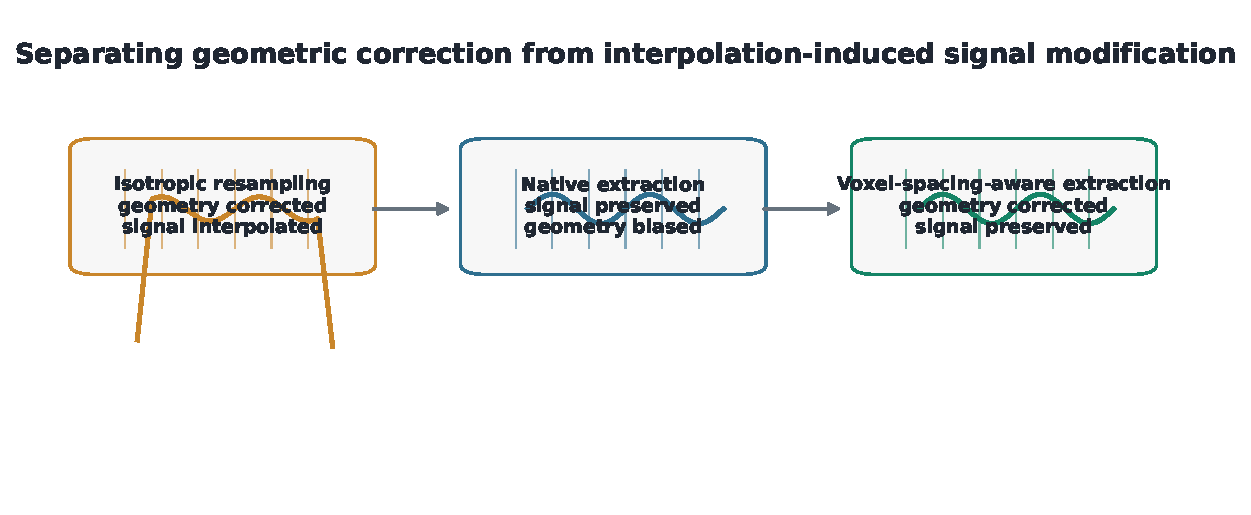
\includegraphics[width=0.95\linewidth]{figures/figure1_conceptual_vs_resampling.pdf}
\caption{Conceptual separation between isotropic resampling and voxel-spacing-aware extraction.}
\label{fig:concept}
\end{figure}

\begin{figure}[H]
\centering
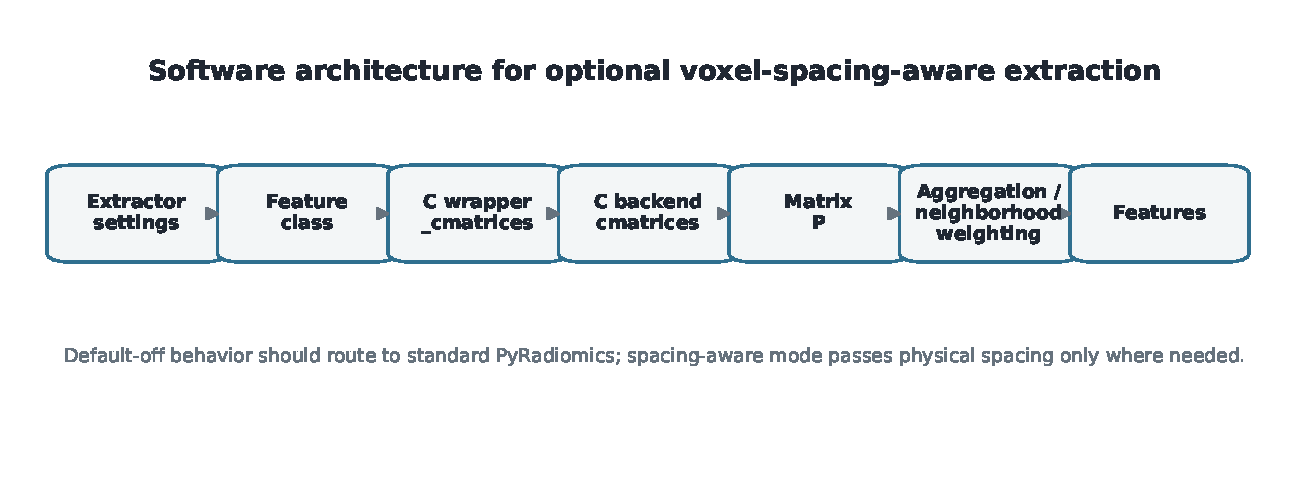
\includegraphics[width=0.95\linewidth]{figures/figure2_software_architecture.pdf}
\caption{Software architecture of the modified PyRadiomics implementation.}
\label{fig:architecture}
\end{figure}

\begin{figure}[H]
\centering
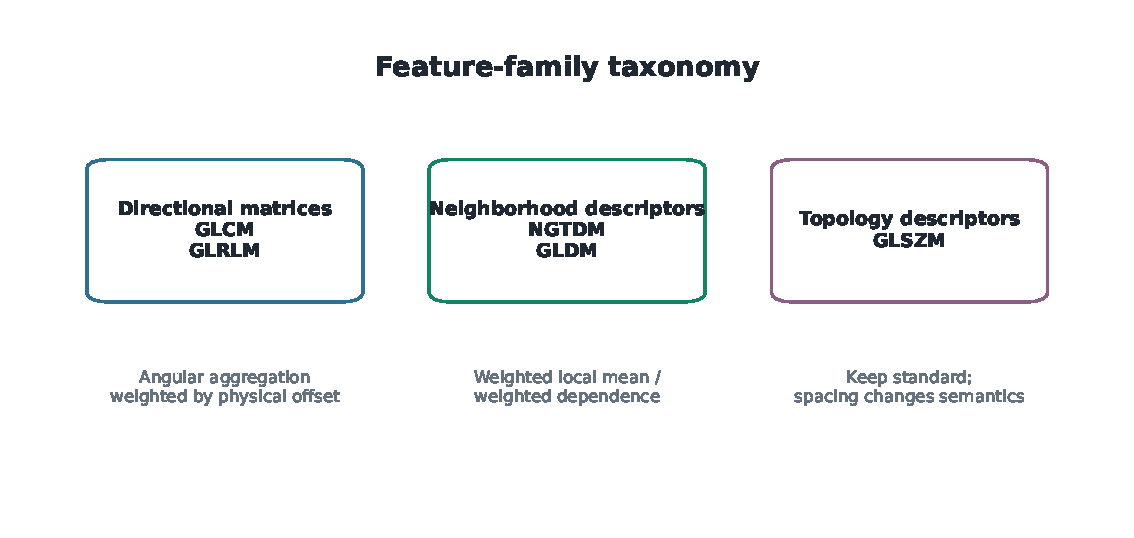
\includegraphics[width=0.95\linewidth]{figures/figure3_feature_taxonomy.pdf}
\caption{Feature-family taxonomy for spacing-aware modifications.}
\label{fig:taxonomy}
\end{figure}

\begin{figure}[H]
\centering
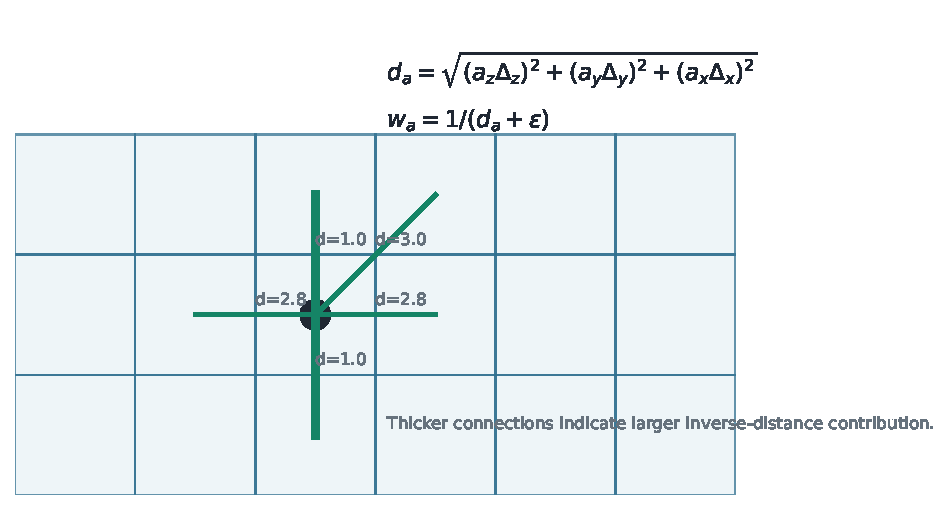
\includegraphics[width=0.85\linewidth]{figures/figure4_physical_offset_weighting.pdf}
\caption{Physical offset weighting in an anisotropic voxel grid.}
\label{fig:weights}
\end{figure}

\begin{figure}[H]
\centering
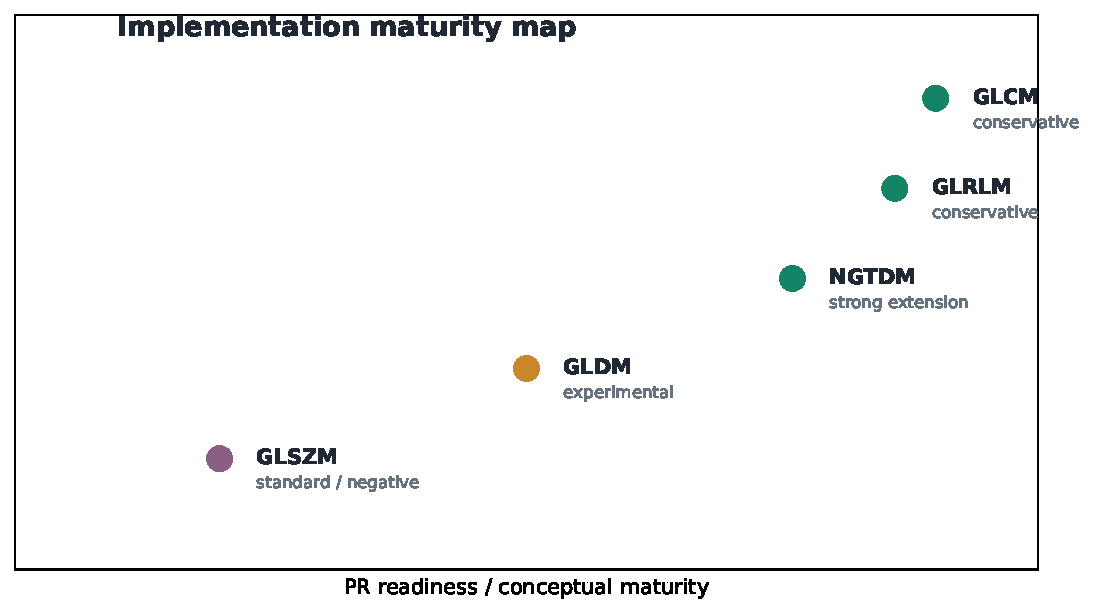
\includegraphics[width=0.95\linewidth]{figures/figure5_pr_maturity_map.pdf}
\caption{Implementation maturity map for a potential upstream pull request.}
\label{fig:maturity}
\end{figure}

\begin{figure}[H]
\centering
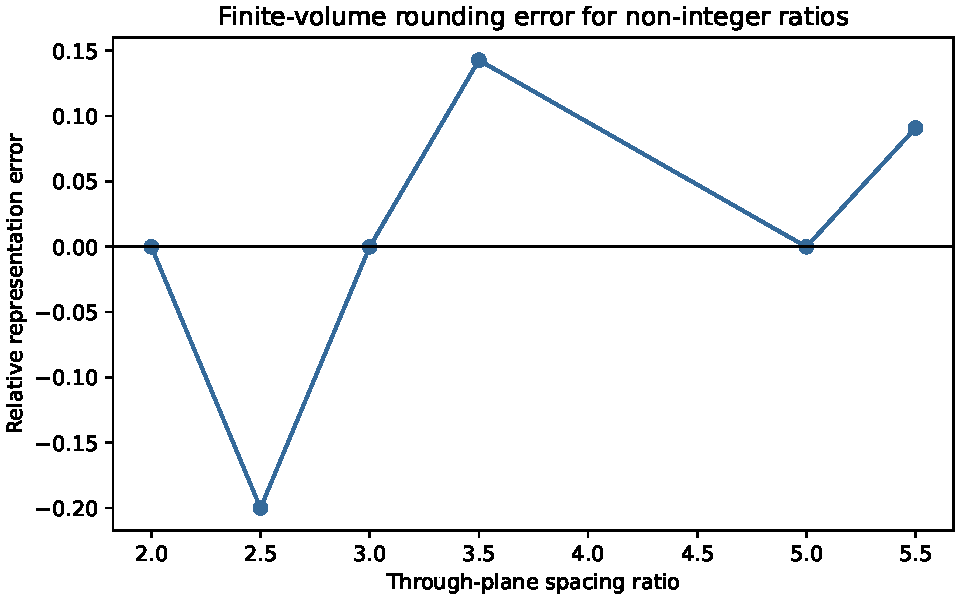
\includegraphics[width=0.95\linewidth]{../experiments/finite_volume_rounding_sensitivity/figures/rounding_error_vs_spacing_ratio.pdf}
\caption{Represented-spacing error introduced by integer finite-volume repeat factors across tested spacing ratios.}
\label{fig:rounding-error}
\end{figure}

\begin{figure}[H]
\centering
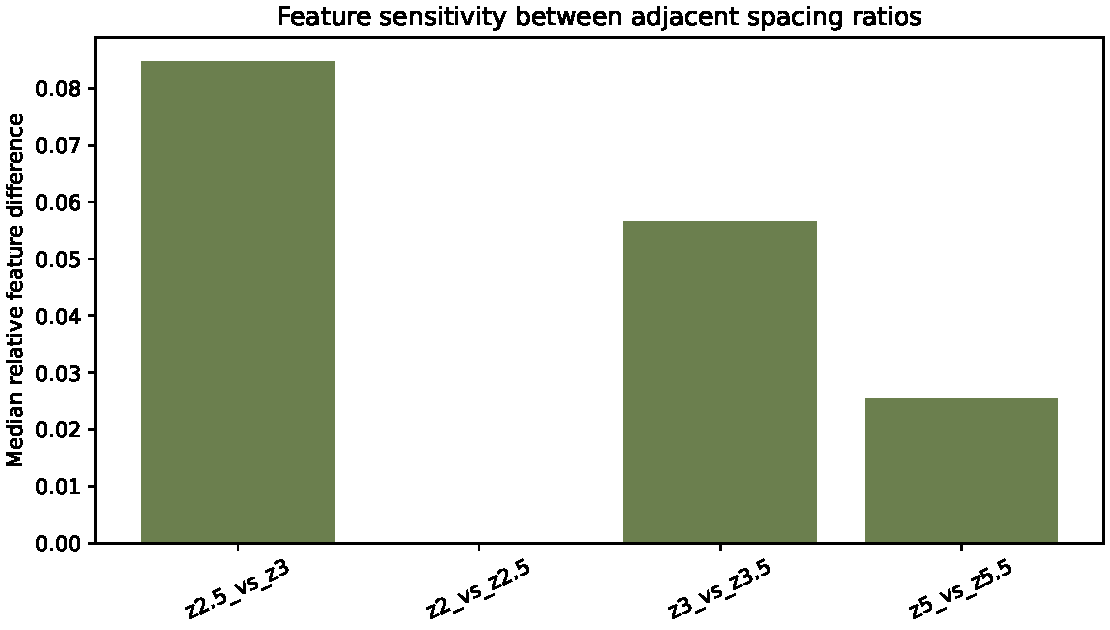
\includegraphics[width=0.95\linewidth]{../experiments/finite_volume_rounding_sensitivity/figures/feature_sensitivity_to_rounding.pdf}
\caption{Family-level feature sensitivity across adjacent integer and non-integer finite-volume spacing ratios.}
\label{fig:rounding-feature-sensitivity}
\end{figure}

\begin{figure}[H]
\centering
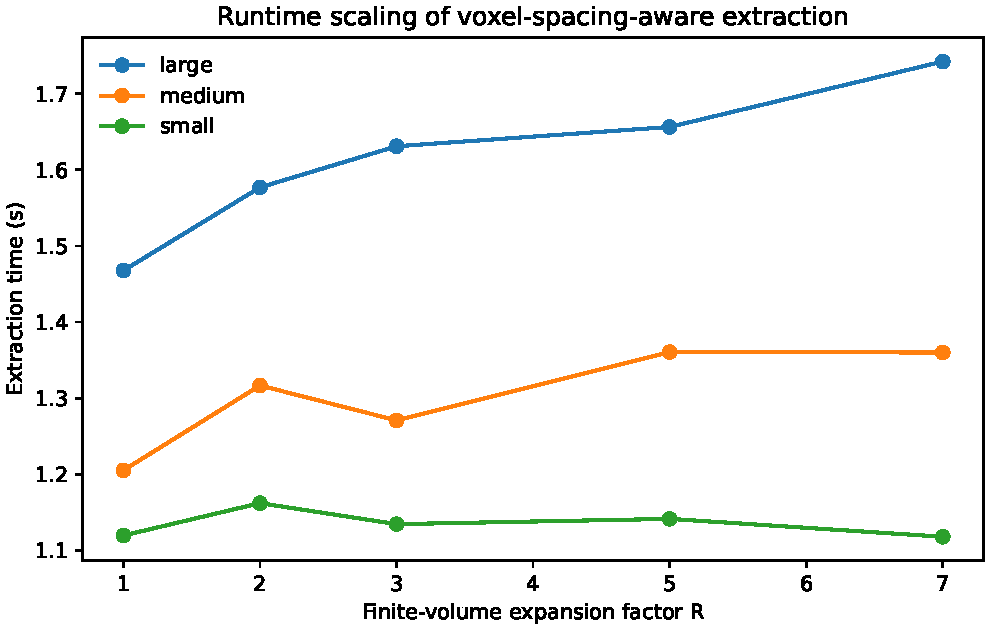
\includegraphics[width=0.95\linewidth]{../experiments/computational_profiling/figures/runtime_vs_expansion_factor.pdf}
\caption{Runtime profile as a function of finite-volume expansion factor in the synthetic stress test.}
\label{fig:runtime-expansion}
\end{figure}

\begin{figure}[H]
\centering
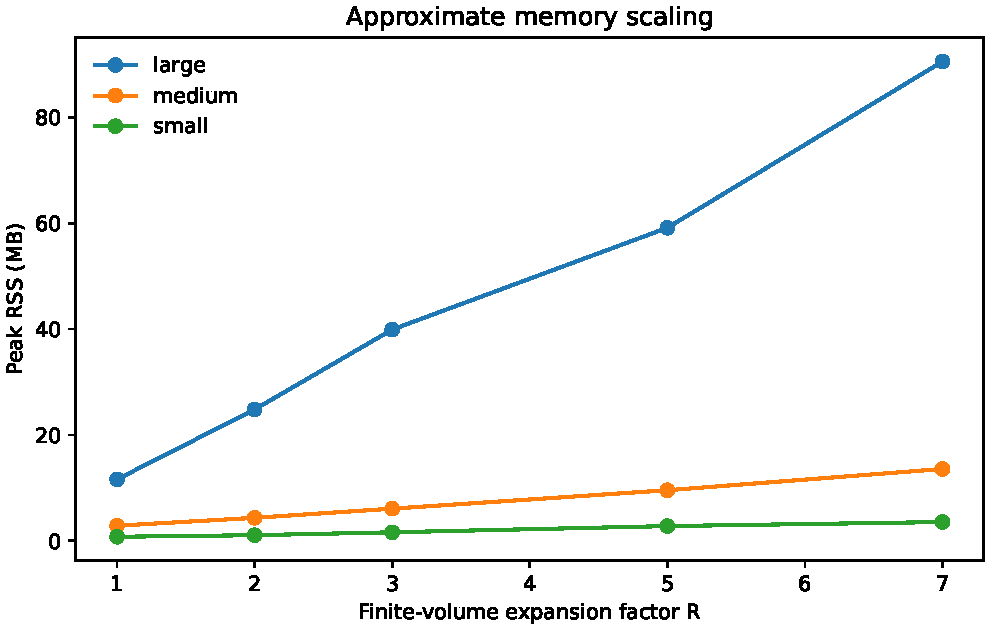
\includegraphics[width=0.95\linewidth]{../experiments/computational_profiling/figures/memory_vs_expansion_factor.pdf}
\caption{Peak memory profile as a function of finite-volume expansion factor in the synthetic stress test.}
\label{fig:memory-expansion}
\end{figure}

\begin{figure}[H]
\centering
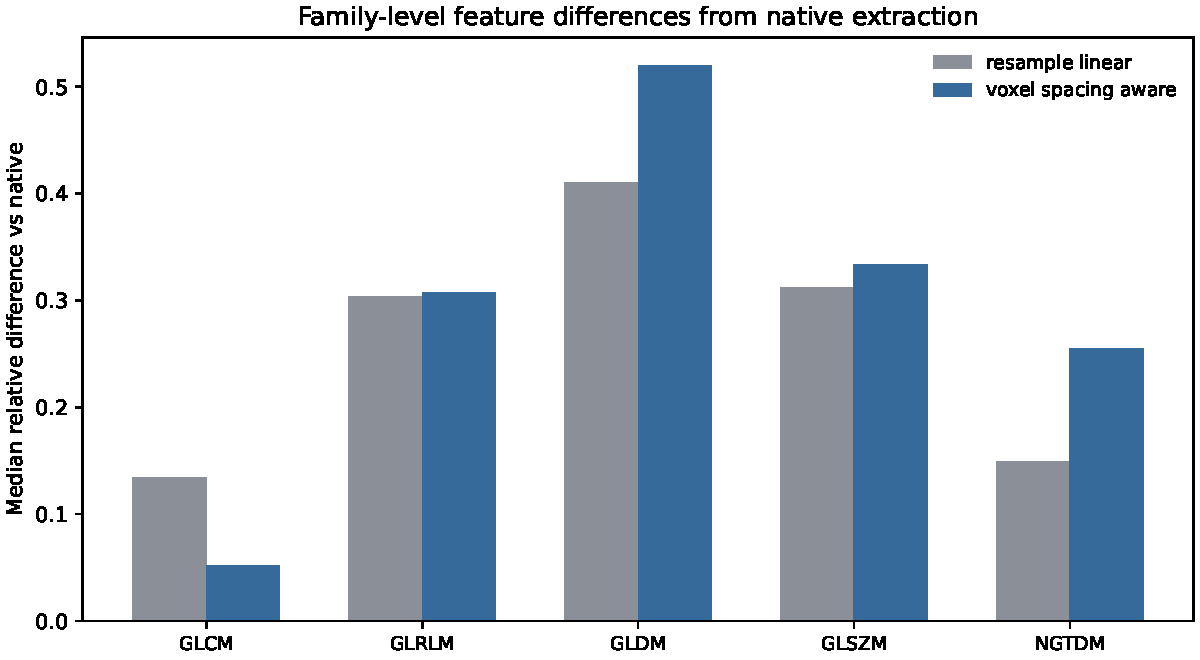
\includegraphics[width=0.95\linewidth]{../experiments/resampling_baseline_comparison/figures/family_relative_difference_barplot.pdf}
\caption{Family-level relative differences from native extraction for nearest-neighbor, linear, B-spline and voxel-spacing-aware extraction.}
\label{fig:resampling-family-differences}
\end{figure}

\begin{figure}[H]
\centering
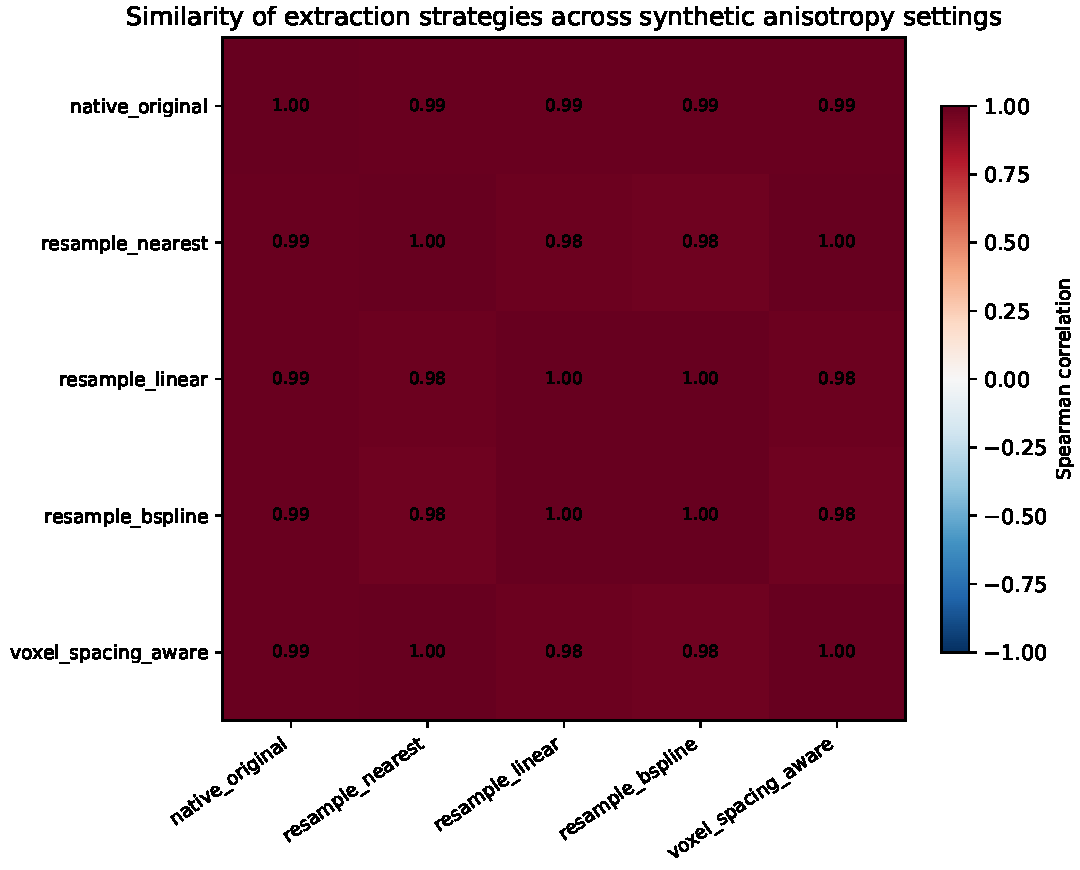
\includegraphics[width=0.95\linewidth]{../experiments/resampling_baseline_comparison/figures/heatmap_method_similarity.pdf}
\caption{Method similarity across native extraction, isotropic resampling baselines and voxel-spacing-aware extraction.}
\label{fig:resampling-method-similarity}
\end{figure}

\end{document}
